\documentclass[a4paper,12pt]{article}
\usepackage{blindtext}
\usepackage[utf8]{inputenc}
\usepackage{graphicx}

\begin{document}
\begin{titlepage}
\center

\textsc{\LARGE Project: Unit-Assess}\\[1.5cm]
\textsc{\Large Client: Mr Schalk Lotz, Magna BC}\\[0.5cm]
\textsc{\large Team: Quadcore Productions}\\[0.5cm]

\begin{minipage}{0.4\textwidth}
\begin{flushleft} \large
\emph{Author(s):}\\
Mpho \textsc{Baloyi}\\
Hlengekile \textsc{Jita}\\
Mayimela \textsc{Moses}\\
Mbhele \textsc{Themba}\\
\end{flushleft}
\end{minipage}
~
\begin{minipage}{0.4\textwidth}
\begin{flushright} \large
\emph{Student number(s):} \\
14133670\\ % Student number
14077893\\
14019702\\
14007950\\
\end{flushright}
\end{minipage}\\

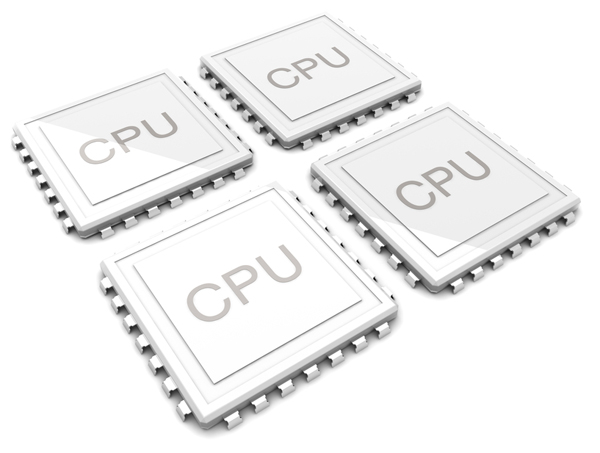
\includegraphics[width=\textwidth]{2012-quad-core-phones}

{\large University of Pretoria, Department of Computer Science}\\

{\large 02 May 2016}\\[3cm]

\vfil

\end{titlepage}

\newpage
\newpage
\tableofcontents
\section{The Team}
\subsection{Mpho Baloyi}
\subsubsection{Interests}
\begin{itemize}
\item Keeping abreast with new technologies
\item Learning and using new technologies to solve problems
\item Reading up and doing research on new and old concepts in computer science
\item Solving riddles and puzzles
\item Helping people through ICT
\end{itemize}
\subsubsection{Technical Skills}
\begin{itemize}
\item Solid programming skills in java,c++ and python
\item Fair amount of knowlegde in assembly programming
\item Web development with HTML,JAVASCRIPT,JQUERY,CSS,PHP,AJAX,ANGULARJS
\item Interaction Design
\item Database design with MySQL
\item Understanding of process development
\item Unit testing,mocking and dependency Injection
\end{itemize}
\subsubsection{Non-Technical Strengths}
\begin{itemize}
\item Excellent Communication skills
\item Patient
\item Creative approach to problem solving
\item Pay attention to detail
\item Excellent planning skills
\item Ability to grasp concepts quickly
\item Willness to learn new things
\item Ability to interpret and follow technical plans
\item Ability to collaborate and work efficiently with other people
\item Ability to work under pressure
\end{itemize}
\subsubsection{Relevant Past Experiences}
Work in the mini-project of the university of Pretoria taught me impoortant skills in software engineering such as unit testing,dependency injection,mocking and working with different technologies. I believe that these skills will be valuable to the development of this project as they apply in every area of software development.
\subsubsection{Reasons for wanting to do the project}
I want to do this project because it provides me with the opportunity to work with different kinds of technologies and devices and to learn new ways of collecting data.
\subsection{Hlengekile Jita}
%\includegraphics[width=\textwidth]{}
\subsubsection{Interests}
\subsubsection{Technical Skills}
\begin{itemize}
\item Microsoft Office - Word, Excel, Access, PowerPoint
\item Programming - Java, C++, Python, Android
\item Database Design - MySQL
\item Web Development - XHTML, HTML5, CSS, JavaScript, PHP
\end{itemize}
\subsubsection{Non-Technical Strengths}
\begin{itemize}
\item Good leader
\item Excellent communication skills both verbal and written
\item Works well under pressure
\item Great at teamwork
\item Sociable character that gets along with people
\item Organized individual with meticulous planning skills
\item Determined
\end{itemize}
\subsubsection{Relevant Past Experiences}
\subsubsection{Reasons for wanting to do the project}
\newpage
\subsection{Moses Mayimela}
\includegraphics[width=\textwidth]{images/moses.jpg}
\subsubsection{Interests}
\begin{itemize}
\item Keeping up to date with the latest technologies e.g Raspberry pi and Intel Edison.
\item Reading Tech reviews and comparisons on software and hardware systems such as BLE vs Classic bluetooth.
\item Taking part in hackerthons e.g Hack4Water.
\end{itemize}
\subsubsection{Technical Skills}
\begin{itemize}
\item Programming skills in:
\begin{enumerate}
\item Java.
\item C for embedded Systems (8 bit and 32 bit) and PC applications.
\item C++.
\item C\#.
\item Python.
\end{enumerate}
\item knowlegde in assembly programming for embedded (8 bit and 32 bit) and PC applications.
\item Web development with
\begin{enumerate}
\item HTML
\item Javascript.
\item NodeJS (Javascript framework)
\item CSS
\item PHP
\item AJAX
\end{enumerate}
\item Database design with MySQL,MSSQL and Postgresql.
\item Unit testing,mocking and dependency Injection
\item Familiar with GSM/3G Modules AT commands.
\item Experience with Linux servers.
\end{itemize}
\subsubsection{Non-Technical Strengths}
\begin{itemize}
\item I like working with people who love what they do.
\item I can lead a team and I also respect a leader.
\item I am always willing to learn and expand my horizons.
\item I am open minded to people's opinions.
\end{itemize}
\subsubsection{Relevant Past Experiences}
\begin{itemize}
\item Won, breakthrough developer award for 2015 in the MTN M2M (IoT) competition.\\
http://www.mind2machine.co.za \\
https://www.youtube.com/watch?v=HZlryrw1Ois.
\item 2nd place at the Hack4Water Hackathon in April 2016.\\
https://twitter.com/hashtag/hack4water
\end{itemize}
Work in the mini-project of the university of Pretoria taught me impoortant skills in software engineering such as unit testing,dependency injection,mocking and working with different technologies. I believe that these skills will be valuable to the development of this project as they apply in every area of software development.
\subsubsection{Reasons for wanting to do the project}
This project will provide an opportunity for me to expand my knowledge in programming while providing a fully functional solution for the client. The technologies in this project will also help me learn better software standards.
\newpage
\subsection{Themba Mbhele}
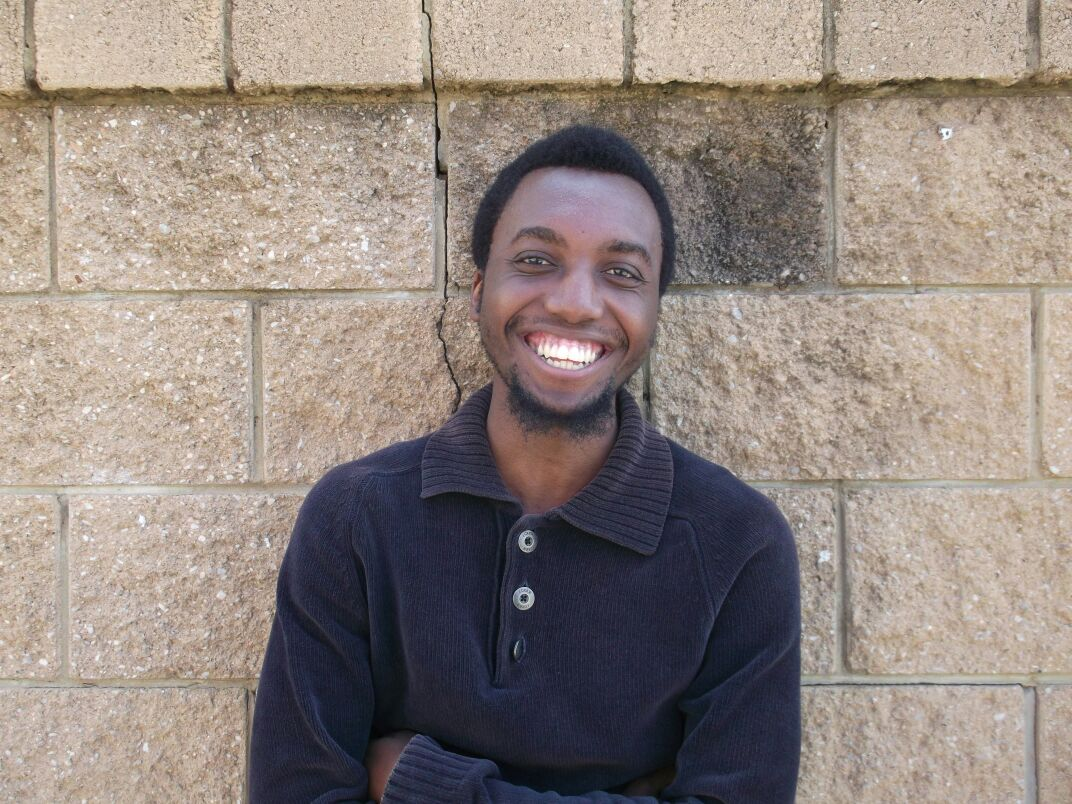
\includegraphics[width=\textwidth]{images/Themba.jpg}
\subsubsection{Interests}
\subsubsection{Technical Skills}
\subsubsection{Non-Technical Strengths}
\subsubsection{Relevant Past Experiences}
\subsubsection{Reasons for wanting to do the project}
\section{Project Execution}
\subsection{Development Methodology}
The project is composed of three core components, the first one being the collection of data from various software systems which is sent to a server, then the programming of the server that will process the information by performing the necessary calculations, and then the design of user interfaces (mobile and web) where the processed data will be displayed to the client.\\
Because our clients happiness is of utmost importance, we have decided to make use of Agile processes. With this approach, we will have deliverables that we will produce on a regular basis and from an early stage. This will facilitate communication between us as the developers and project owner, Mr Schalk Lotz of Magna BC, so that we may work together to develop a high quality system.\\
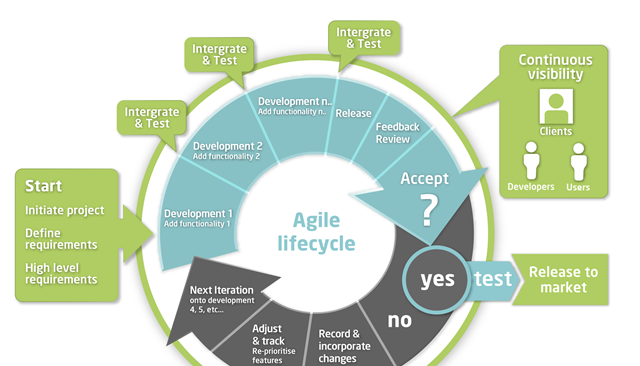
\includegraphics[width=\textwidth]{images/agileDev.png}
\subsection{Communication With Client}
To keep the clients informed we are going to use the following means of communication
\subsubsection{email}
\begin{itemize}
\item To inform the client of our progress
\item To address any issues or concerns that they client may have
\item To acquire information from the client
\item To require any resources that the client has to offer for their project,..
\end{itemize}
\subsubsection{Regular Meetings}
These will take place depending on the clients availability and willingness.
We may discuss the progress of the project,to address any concerns,etc.
\subsubsection{GIT}
Access to our git repository will be provided to the client,so the client can be able to monitor
our progress and have access to the project material.
We are also open to any means of communication that the client may prefer or suggest.
\subsection{Technical Challenges}
\subsubsection{Dealing with a wide range of information sources}
As described in the project proposal, the automated performance management system is required to assess the performance of staff based on information sourced across different software systems. The measuring of performance should be done across a configurable range of performance areas.\\

This presents the technical challenge of dealing with a wide range of information sources. This is a challenge because information from various sources will come in various formats and our system would need to be able to process this information. Especially if the range is configurable, the system needs to be able to deal with new sources of information that may not have been considered during initial development.\\

The solution for this would be to have the system deal with all sources of information in the same way. This can be done through making use of the software design pattern, dependency injection. This will help us apply inversion of control for resolving the dependency of the system on an information source. By passing the system the information source in a standard format through interface based injection, instead of having the system have to understand a wide range of information sources so that it can work with each one, we are able to focus on the information processing rather than each possible information source.

\subsubsection{Determining Performance Criteria}
Performance will be measured and then aggregated through this system. Aggregation can either be by weighted average or best-n based. Considering that information will come from a wide range of sources, the question arises of how the criteria will be specified. \\
There are two possibilities:
\begin{itemize}
\item The client can specify a standard that will be applied across the board, i.e. information from certain kind's of sources will always carry more weight than others. The system will always calculate performance the same way despite the specific context of use.
\item Or the client or any user of the system will be able to specify which sources they want to track performance from and specify the criteria to be applied and the system is able to adapt accordingly and perform assessments appropriately. 
\end{itemize}
The latter option, is the preferred solution because it will be then possible to apply the system across a wide range of contexts. The system could be applied in an endless range of environments.
\section{Technologies}
\subsection{Server: GlassFish}
The choice of technologies is mostly guided by the client.These are:\\
GlassFish, this is an open source java framework for java servlets.
\subsection{Database:MySql}
MySql, open source database server.It is robust and has a large community of developers for support.
Database transactions will be handled using JPA for persisting data.
\subsection{Data transactions:JPA}
For data exchange, JPA will be used to allow access to the database in an object oriented way.
\subsection{Android development}
The Android SDK will be used for the Android application. The SDK is open-source and well supported by a large community od developers.
\subsection{Front end interface: Ember.js}
As already specified in the project proposal, Ember.js will be used for the front-end development.

\end{document}
